\subsubsection{Login}
The user must login onto the page for the user to be able to participate in a session. There are two alternatives login methods the user can choose between. Preferably for the user, the user can log onto the page using their Feide user. If the user chooses this method, then the user has access to any previous questions and given answers to the sessions the user has participated in. The user also does not need to worry about losing data if the user disconnects from the application. However, cookies are used in this login method. Alternatively, the user can login anonymously, which does not require the usage of cookies on the client. It does however, mean that the user does not have access to any previous question data, and if the user disconnects, then the user must go through the entire login process again. The following steps are used for the user to login onto the page, both alternatives are listed:
\paragraph{Anonymous Login}
\begin{enumerate}
	\item Assuming the user has managed to enter the home page of the application, the user needs to click on the Sign in button in right 				  corner of the navigation bar, to enter the login page.\ref{fig:annoMainPage}
	\item Next the user must verify the login method. Anonymous is chosen as the default login method, therefore this step can be skipped 				  unless the user has previously clicked the “Feide” button If this case, then user has to click on the button labeled “Anonymous”.\ref{fig:annoLogin}
	\item Finally the user must click on the button labeled “Sign in” to anonymously log onto the page.\ref{fig:annoLogin} If the login was 			  successful, the user is redirected to the /client page and the button labeled “Sign in” on the navigation bar is displaying a random 		  anonymous animal name.\ref{fig:annoResult}
\end{enumerate}
\begin{figure}[H]
    \centering
    \begin{subfigure}{0.60\linewidth}
        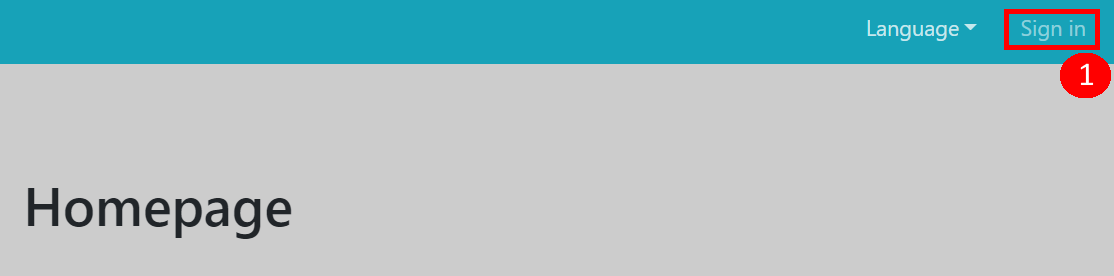
\includegraphics[width=\linewidth]{/userManual/login/mainpage}
       	\caption{Figure displays main page off the application. Step 1. is visible in the figure.}
		\label{fig:annoMainPage}	
    \end{subfigure}
    \begin{subfigure}{0.60\linewidth}
        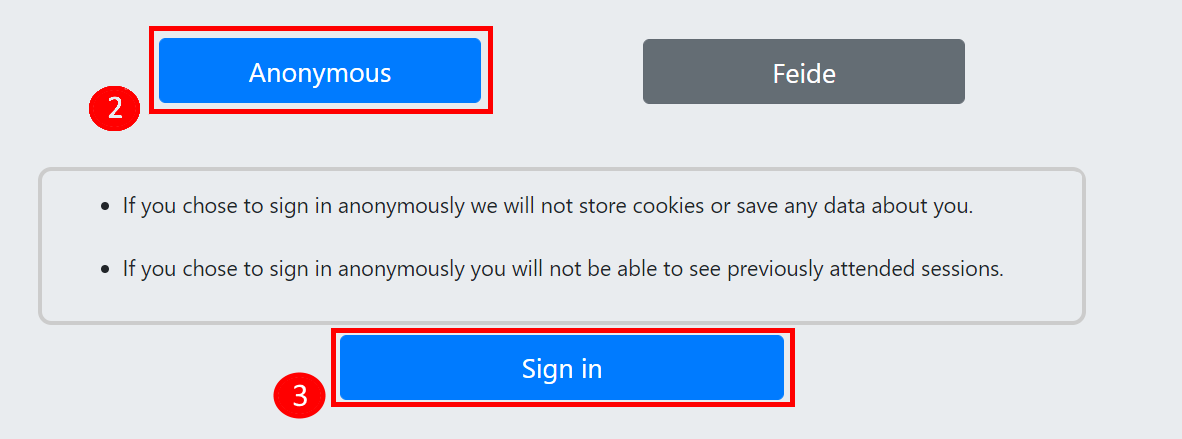
\includegraphics[width=\linewidth]{/userManual/login/annoLogin}
      	\caption{Figure displays login page when anonymous method is chosen. Step 2. and 3. are visible in the figure.}
		\label{fig:annoLogin}	
    \end{subfigure}
    \begin{subfigure}{0.60\linewidth}
    	
\includegraphics[width=\linewidth]{/userManual/login/annoResult}
    	\caption{Figure displays the navigation bar after the user has logged onto the Application anonymously. In this case the name "humpback whale" is the random animal name assigned which was assigned to the user.}
    	\label{fig:annoResult}	
    \end{subfigure}
\end{figure}
\paragraph{Feide Login}
\begin{enumerate}
	\item Assuming the user has managed to enter the home page of the application, the user needs to click on the Sign in button in right corner of the navigation bar, to enter the login page.\ref{fig:feideMainPage}
	\item Next the user must verify the login method. In this case, the user needs to click on the button labeled as “Feide”. Once the user has clicked on this button the sites terms of use will be updated with the application use of cookies.\ref{fig:feideLogin}
	\item After the user has read through the web applications terms of use, the user needs to verify that they have accepted these terms by checking the radio button. Once this is done, the radio button gets a blue background and the button labeled “Sign in” is no longer disabled.\ref{fig:feideLogin}
 	\item Finally the user must click on the button labeled “Sign in” to log onto the page with their Feide account.\ref{fig:feideLogin} The user is then redirected to Uninett, where the user has to sign into their Feide account. Once this is done the user is redirected to the applications client page. If the login was successful if and the button labeled “Sign in” on the navigation bar is now displaying the users Feide username.\ref{fig:feideResult}
\end{enumerate}
\begin{figure}[H]
    \centering
    \begin{subfigure}{0.60\linewidth}
        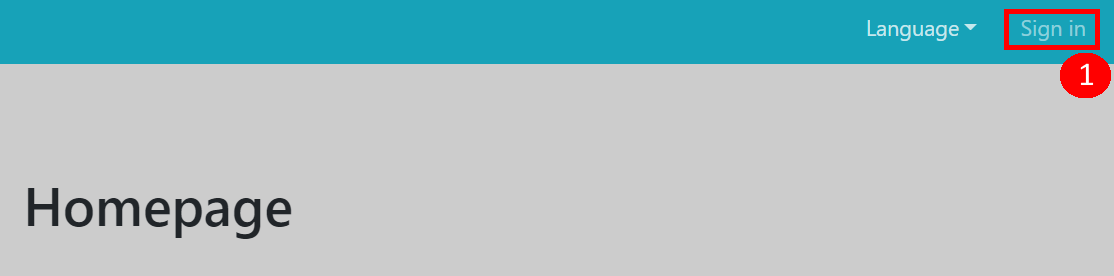
\includegraphics[width=\linewidth]{/userManual/login/mainpage}
       	\caption{Figure displays main page off the application. Step 1. is visible in the figure.}
		\label{fig:feideMainPage}	
    \end{subfigure}
    \begin{subfigure}{0.60\linewidth}
        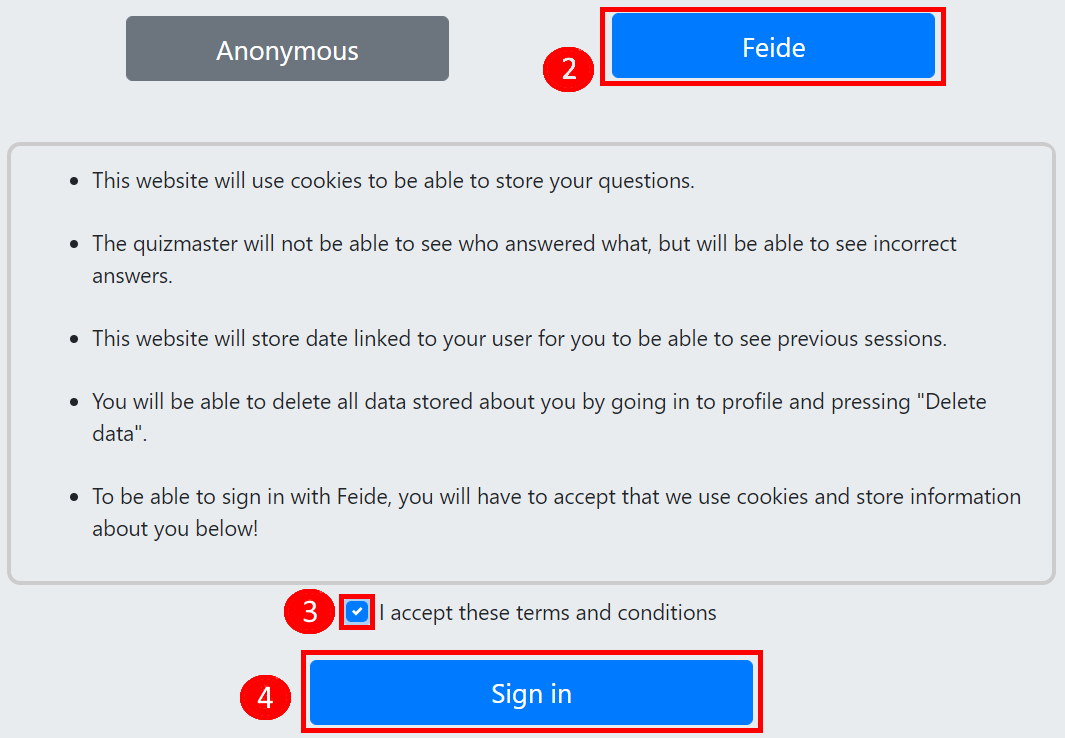
\includegraphics[width=\linewidth]{/userManual/login/feideLogin}
      	\caption{Figure displays login page when Feide method is chosen. Step 2., 3. and 4. are visible in the figure.}
		\label{fig:feideLogin}	
    \end{subfigure}
     \begin{subfigure}{0.60\linewidth}
        
\includegraphics[width=\linewidth]{/userManual/login/feideResult}
      	\caption{Figure displays the navigation bar after the user has logged onto the Application with their Feide user.}
		\label{fig:feideResult}	
    \end{subfigure}
\end{figure}